\chapter{\IfLanguageName{dutch}{Resultaten enquête}{Resultaten enquête}}
\label{ch:Resultaten_enquête}

Hieronder vindt u alle resultaten van elke vraag in de enquête. De resultaten uit de enquête zijn uiterst relevant voor dit onderzoek, deze werden gebruikt voor het vinden van een antwoord op dit onderzoek. Daarbij is het belangrijk om te weten dat wanneer u bij de tabellen 'overige' ziet staan. Dit betekent dat deze vragen niet zijn ingevuld. M.a.w. zijn dit de personen die niet gekend zijn met Cisco Identity Services Engine. Met als gevolg dat voor hun deze vragen niet zichtbaar waren.
\newline

\textbf{Vraag 1 : Ken u Cisco Identity Services Engine?}
\begin{table}[h!]
\begin{center}
		\begin{tabular}{|l|l|}
			\hline
			\bf Antwoorden    & \bf Percentages \\ \hline
			Ja  & 78.6\% \\ \hline
			Nee & 21.4\% \\ \hline
		\end{tabular}
	\caption{Resultaat vraag 1.}
\end{center}
\end{table}

\newpage
\textbf{Vraag 2: Waar heeft u voor het eerst gehoord van Cisco Identity Services Engine?}
\begin{table}[H]
	\begin{center}
		\begin{tabular}{|l|l|}
			\hline
			\bf Antwoorden    & \bf Percentages \\ \hline
			Tijdens een webinair   & 7.2\%  \\ \hline
			Tijdens een opleiding  & 7.2\%  \\ \hline
			In de organisatie      & 71.4\% \\ \hline
			Op het internet        & 7.2\%  \\ \hline
			Op een reclame campage & 0\%    \\ \hline
			Op televisie           & 0\%    \\ \hline
			Andere                 & 0\%    \\ \hline
		\end{tabular}
		\caption{Resultaat vraag 2.}
	\end{center}
\end{table}

\textbf{Vraag 3: Wordt Cisco Identity Services Engine binnen uw organisatie toegepast?}

\begin{table}[h!]
	\begin{center}
		\begin{tabular}{|l|l|}
			\hline
		\bf Antwoorden    & \bf Percentages \\ \hline
		Ja      & 78.6\% \\ \hline
		Nee     & 0\%    \\ \hline
		Overige & 21.4\% \\ \hline
		\end{tabular}
		\caption{Resultaat vraag 3.}
	\end{center}
\end{table}

\textbf{Vraag 4: Wordt er een network access control product gebruikt in uw organisatie? }

\begin{table}[h!]
	\begin{center}
		\begin{tabular}{|l|l|}
			\hline
			\bf Antwoorden    & \bf Percentages \\ \hline
			Ja      & 0\%   \\ \hline
			Nee     & 100\% \\ \hline
			Overige & 0\%   \\ \hline
		\end{tabular}
		\caption{Resultaat vraag 4.}
	\end{center}
\end{table}

Dit werd ingevuld door de personen die niet gekend zijn met Cisco Identity Services Engine.
\\ \textbf{Vraag 5: Welk network access control product wordt in uw organisatie gebruikt?}

\begin{table}[h!]
	\begin{center}
		\begin{tabular}{|l|l|}
			\hline
			\bf Antwoorden \\ \hline
			/ \\ \hline
		\end{tabular}
		\caption{Resultaat vraag 5.}
	\end{center}
\end{table}

\newpage
\textbf{Vraag 6: Met welke reden werd Cisco Identity Services gekozen als network access control in uw bedrijfsomgeving?}
\begin{table}[H]
	\begin{center}
		\begin{tabular}{|l|l|}
			\hline
			\bf Antwoorden    & \bf Percentages \\ \hline
			Omwille van Cisco's bedrijfsimago.                                                   & 18.75\% \\ \hline
			Omwille van de betere bescherming tegen interne of externe threads.                  & 12.50\% \\ \hline
			Omwille van de betere zichtbaarheid/nauwkeurigheid voor apparaatidentificatie.       & 18.75\% \\ \hline
			Omwille van de betere beheerbaarheid van end-point systemen.                         & 31.25\% \\ \hline
			Andere                                                                               & 18.75\% \\ \hline                                                        
		\end{tabular}
		\caption{Resultaat vraag 6.}
	\end{center}
\end{table}

\begin{table}[h!]
	\begin{center}
		\begin{tabular}{|l|l|}
			\hline
			\bf Antwoorden    & \bf Percentages \\ \hline
			Eenvoudige integratie met andere Cisco producten.                        & 33.33\% \\ \hline
			Goede marketing van Cisco.                                                             & 33.33\% \\ \hline
			Standaardisatie op producten binnen het Cisco Ecosysteem. & 33.33\% \\ \hline
		\end{tabular}
		\caption{Redenen van het antwoord: 'Andere'.}
	\end{center}
\end{table}

\textbf{Vraag 7: Welke kernmerken zijn volgens u belangrijk om te kiezen voor een network access control product?}
\begin{table}[h!]
	\begin{center}
		\begin{tabular}{|l|l|l|l|}
			\hline
			\bf Antwoorden          & \multicolumn{3}{l|}{\bf Percentages} \\ \hline
					 			  				  & Onbelangrijk & Neutraal & Belangrijk \\ \hline
			Prijs                                 & 9.1\%        & 45.5\%   & 45.4\%     \\ \hline
			Functionaliteit                       & 0\%          & 9.1\%    & 90.9\%     \\ \hline
			Uitbreidbaarheid                      & 0\%          & 18.2\%   & 81.8\%     \\ \hline
			Beleidshandhaving                     & 0            & 9.1      & 90.9\%     \\ \hline
			Identiteits- en toegangsbeheer        & 0\%          & 0\%      & 100\%      \\ \hline
			Automatisatie                         & 0\%          & 45.5\%   & 54.5\%     \\ \hline
			Verificatie, autorisatie, boekhouding & 0\%          & 36.4\%   & 63.6\%     \\ \hline
			Minder bedreigingen                   & 0\%          & 27.3\%   & 72.7\%     \\ \hline
			Gemakkelijk te configureren           & 9.0\%        & 45.5\%   & 45.5\%     \\ \hline
			Bedrijfsimago                         & 27.2\%       & 36.4\%   & 36.4\%     \\ \hline
			Eenvoud                               & 9.1\%        & 54.6\%   & 36.3\%     \\ \hline
		\end{tabular}
		\caption{Resultaat vraag 7.}
	\end{center}
\end{table}

\newpage
\textbf{Vraag 8: Ondervond u na de implementatie van Cisco Identity Services Engine enige veranderingen? Zoja, welke?}
\begin{table}[H]
	\begin{center}
		\newlength\q
		\setlength\q{\dimexpr 1\textwidth}
		\noindent\begin{tabular}{p{\q}p{\q}}	
		\hline
		\bf Antwoorden \\ \hline
		Dankzij ISE kunnen we tenminste weten wie er op ons netwerk geconnecteerd is, en er zeker van zijn dat er geen onbekenden op zitten.                                                                       \\ \hline
		Nee                                                                                                                                                                                                        \\ \hline
		downside: minder flexibiliteit \& eenvoud op netwerk configatie gebied, maar elke security oplossing is het evenwicht zoeken tussen veiligheid, usability \& kostprijs. De Peace of mind is ook wat waard. \\ \hline
		Niet aantoonbaar                                                                                                                                                                                           \\ \hline
		Makkelijker troubleshooten van authenticatie problemen + makkelijk auditen van wie op welke netwerk device aan het werken is.                                                                              \\ \hline
		We hadden alle controle terug over onze poorten. Een onbekend toestel werd gesinkholed, tot frustratie van de eindgebruiker maar vanuit een security standpunt een droom.                                  \\ \hline
		Sinds de implementatie is het duidelijk welke apparaten met het netwerk verbonden zijn. \\ \hline
		\end{tabular}
		\caption{Resultaat vraag 8.}
	\end{center}
\end{table}

\textbf{Vraag 9: Wat vindt u van de kwaliteit van Cisco Identity Services Engine t.o.v. andere network access control producten?}
\begin{table}[h!]
	\begin{center}
		\begin{tabular}{|l|l|}
			\hline
			\bf Antwoorden    & \bf Percentages \\ \hline
			Veel beter    & 0\%    \\ \hline
			Beter         & 36.4\% \\ \hline
			Gelijkaardig  & 54.5\% \\ \hline
			Slechter      & 9.1\%  \\ \hline
			Veel slechter & 0\%    \\ \hline                                                                                                                                 
		\end{tabular}
		\caption{Resultaat vraag 9.}
	\end{center}
\end{table}

\newpage
\textbf{Vraag 10: Wat zijn volgens u de meeste voorkomende modules of use cases van Cisco Identity Services Engine?}

\begin{table}[H]
	\begin{center}
		\begin{tabular}{|l|l|}
			\hline
			\bf Antwoorden          & \bf Percentages \\ \hline
			Policy-Based AC     & 34.6\%      \\ \hline
			Per-user dynamic AC & 7.7\%       \\ \hline
			Thread-centric AC   & 11.5\%      \\ \hline
			Identity-Based AC   & 38.5\%      \\ \hline
			Port-Based AC       & 7.7\%       \\ \hline
			Location-Based AC   & 0\%         \\ \hline
			Andere              & 0\%         \\ \hline                                                        
		\end{tabular}
		\caption{Resultaat vraag 10.}
	\end{center}
\end{table}

\textbf{Vraag 11: Welke voordelen heeft Cisco Identity Services Engine binnen een netwerk?}

\begin{table}[H]
	\begin{center}
		\setlength\q{\dimexpr 1\textwidth}
		\noindent\begin{tabular}{p{\q}p{\q}}
		\hline
		\bf Antwoorden                                                                                                                              \\ \hline
		Dynamic host blocking (stealthwatch)                                                                                                         \\ \hline
		Verhoogde security (Authorized access only) en na opzet een verlaagde werklast voor IT (automatisatie van access poort configuratie dmv ISE) \\ \hline
		Je weet wat er op uw netwerk zit                                                                                                             \\ \hline
		koppeling van connectivity \& authentication/identity op de LAN laag in een IT infrastructuur                                                \\ \hline
		Makkelijk authtenticatie en gebruiksvriendelijk guest portal                                                                                 \\ \hline
		Elke poort op elke switch is dezelfde geconfigureerd.  Niet meer zitten klungelen met vlans. Single plane off glass voor management.         \\ \hline
		Introductie van Thread-centric NAC bracht heel wat voordelen naar boven.                                                                     \\ \hline
		Integratie met andere Cisco producten                                                                                                        \\ \hline                                                        
		\end{tabular}
		\caption{Resultaat vraag 11.}
	\end{center}
\end{table}

\textbf{Vraag 12: Heeft Cisco Identity Services Engine ook nadelen binnen een netwerk?}

\begin{table}[h!]
	\begin{center}
		\begin{tabular}{|l|l|}
			\hline
			\bf Antwoorden    & \bf Percentages \\ \hline
			Ja      & 54.5\% \\ \hline
			Nee     & 45.5\%    \\ \hline                                                      
		\end{tabular}
		\caption{Resultaat vraag 12.}
	\end{center}
\end{table}

\newpage
\textbf{Vraag 13: Welke nadelen ondervond u dan?}
\begin{table}[H]
	\begin{center}
		\setlength\q{\dimexpr 1\textwidth}
		\noindent\begin{tabular}{p{\q}p{\q}}
			\hline
		\bf Antwoorden \\ \hline
		Certificate updates require nac to shut down. \\ \hline
		Het netwerk wordt voor een groot stuk afhankelijk van de beschikbaarheid van ISE. Veel meer dan enkele uren downtime van ISE kunnen niet overleefd worden. Dit is vooral nadelig indien men veel kleine Kantoren heeft(waar het niet kostenbaten is om een PSN te zetten). \\ \hline
		Je netwerk is afhankelijk van de nac oplossing.  \\ \hline
		Hogere workeffort bij LAN opzet + hoger aantal support cases. \\ \hline
		Instabiliteit van connecties met sommige systemen. \\ \hline
		De gebruikers kennen dit niet. En verwachten als hun laptop kunnen gebruiken op die switchpoort ze ook hun raspberry pi of PLC kunnen daarop aansluiten.       \\ \hline                                                  
		\end{tabular}
		\caption{Resultaat vraag 13.}
	\end{center}
\end{table}

\textbf{Vraag 14: Is volgens u Cisco Identity Services Engine een logische keuze t.o.v. andere network access control producten?} 

\begin{table}[H]
	\begin{center}
		\begin{tabular}{|l|l|}
			\hline
			\bf Antwoorden    & \bf Percentages \\ \hline
			Ja      & 90.9\% \\ \hline
			Nee     & 9.1\%    \\ \hline                                                           
		\end{tabular}
		\caption{Resultaat vraag 14.}
	\end{center}
\end{table}

\textbf{Vraag 15: Is volgens u een network access control product noodzakelijk in een bedrijfsomgeving?}

\begin{table}[h!]
	\begin{center}
		\begin{tabular}{|l|l|}
			\hline
\bf Antwoorden    & \bf Percentages \\ \hline
Ja      & 100\% \\ \hline
Nee     & 0\%    \\ \hline                                                                               & 18.75\% \\ \hline                                                        
		\end{tabular}
		\caption{Resultaat vraag 15.}
	\end{center}
\end{table}

\textbf{Vraag 16: Ontbreken er volgens u functionaliteiten in Cisco Identity Services Engine?}

\begin{table}[h!]
	\begin{center}
		\begin{tabular}{|l|l|}
		\hline
		\bf Antwoorden    & \bf Percentages \\ \hline
		Ja      & 18.2\% \\ \hline
		Nee     & 81.2\%    \\ \hline                                                         
		\end{tabular}
		\caption{Resultaat vraag 16.}
	\end{center}
\end{table}

\textbf{Vraag 17: Welke functionaliteiten ontbreken er dan?}

\begin{table}[H]
	\begin{center}
		\begin{tabular}{|l|l|}
			\hline
		\bf Antwoorden                                                                        \\ \hline
		Industriële gerichtheid, incl. Goede support voor static IP adressen              \\ \hline
		Saml integratie dit in samenwerking met Azure AD met de Captive portal voor byod. \\ \hline                                                      
		\end{tabular}
		\caption{Resultaat vraag 17.}
	\end{center}
\end{table}

\textbf{Vraag 18: Welke functionaliteiten ontbreken er dan?}
\begin{table}[H]
	\begin{center}
		\begin{tabular}{|l|l|}
			\hline
			\bf Gemiddelde beoordeling                                                                        \\ \hline
			3.91/5 \\ \hline                                                   
		\end{tabular}
		\caption{Resultaat vraag 18.}
	\end{center}
\end{table}

\textbf{Vraag 19: Zou u dit product aanbevelen aan anderen?}

\begin{table}[h!]
	\begin{center}
		\begin{tabular}{|l|l|}
					\hline
			\bf Antwoorden    & \bf Percentages \\ \hline
			Ja      & 90.9\% \\ \hline
			Nee     & 9.1\%    \\ \hline                                                                                                                           
		\end{tabular}
		\caption{Resultaat vraag 19.}
	\end{center}
\end{table}

\textbf{Vraag 20: Heeft u al gehoord van een network access control?}

\begin{table}[h!]
	\begin{center}
		\begin{tabular}{|l|l|}
		\hline
		\bf Antwoorden    & \bf Percentages \\ \hline
		Ja      & 0\% \\ \hline
		Nee     & 100\%    \\ \hline                                                      
		\end{tabular}
		\caption{Resultaat vraag 20.}
	\end{center}
\end{table}

\begin{figure}[H]
	\centering
	\includegraphics[height=0.30\textheight]{Vraag1.png}
	\caption{Deze afbeelding geeft de service 'Wired AutoConfig' weer.}
\end{figure}

\begin{figure}[H]
	\centering
	\includegraphics[height=0.30\textheight]{Vraag2.png}
	\caption{Deze afbeelding geeft de service 'Wired AutoConfig' weer.}
\end{figure}

\begin{figure}[H]
	\centering
	\includegraphics[height=0.40\textheight]{Vraag3.png}
	\caption{Deze afbeelding geeft de service 'Wired AutoConfig' weer.}
\end{figure}

\begin{figure}[H]
	\centering
	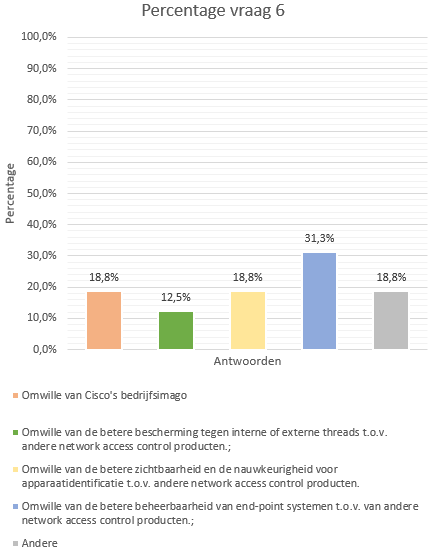
\includegraphics[height=0.30\textheight]{Vraag6.png}
	\caption{Deze afbeelding geeft de service 'Wired AutoConfig' weer.}
\end{figure}

\begin{figure}[H]
	\centering
	\includegraphics[height=0.30\textheight]{Vraag7.png}
	\caption{Deze afbeelding geeft de service 'Wired AutoConfig' weer.}
\end{figure}

\begin{figure}[H]
	\centering
	\includegraphics[height=0.30\textheight]{Vraag9.png}
	\caption{Deze afbeelding geeft de service 'Wired AutoConfig' weer.}
\end{figure}

\begin{figure}[H]
	\centering
	\includegraphics[height=0.30\textheight]{Vraag10.png}
	\caption{Deze afbeelding geeft de service 'Wired AutoConfig' weer.}
\end{figure}

\begin{figure}[H]
	\centering
	\includegraphics[height=0.30\textheight]{Vraag12.png}
	\caption{Deze afbeelding geeft de service 'Wired AutoConfig' weer.}
\end{figure}
\begin{figure}[H]
	\centering
	\includegraphics[height=0.30\textheight]{Vraag14.png}
	\caption{Deze afbeelding geeft de service 'Wired AutoConfig' weer.}
\end{figure}
\begin{figure}[H]
	\centering
	\includegraphics[height=0.30\textheight]{Vraag15.png}
	\caption{Deze afbeelding geeft de service 'Wired AutoConfig' weer.}
\end{figure}
\begin{figure}[H]
	\centering
	\includegraphics[height=0.30\textheight]{Vraag16.png}
	\caption{Deze afbeelding geeft de service 'Wired AutoConfig' weer.}
\end{figure}
\begin{figure}[H]
	\centering
	\includegraphics[height=0.30\textheight]{Vraag19.png}
	\caption{Deze afbeelding geeft de service 'Wired AutoConfig' weer.}
\end{figure}
\begin{figure}[H]
	\centering
	\includegraphics[height=0.30\textheight]{Vraag20.png}
	\caption{Deze afbeelding geeft de service 'Wired AutoConfig' weer.}
\end{figure}
